\chapter{Deep learning in natural language processing} \label{Deep learning in natural language processing}
Deep learning is a branch of machine learning and a re-branded name for neural networks.
All of machine learning can be defined as learning to predict the future based on past observations.
In addition to learning to predict, deep learning also tries to represent the data in such a form that it is suitable for prediction.
Given a large amount of desired input-output mappings, deep learning feeds the data into a network that successively transforms the data until a final transformation predicts the output.
The transformations are learned from the mappings such that each successive transformation makes it easier to relate the data to the given label.
After a human designer defines the architecture and training regime of the network, gathers and preprocesses a proper set of input-output examples and encodes the data, the network can automatically learn how to best produce this mapping \cite{goldberg2017}.

This chapter gives an overview of transfer learning in section \ref{Transfer learning}, delves deeper into how a deep learning model is trained in section \ref{Training}, provides an overview of different relevant architectures in section \ref{Architectures} and finally describes the methodology of three modern machine learning models: ULMFit, BERT and ELECTRA, in section \ref{Modern models}.

\section{Transfer learning} \label{Transfer learning}
Transfer learning refers to the ability of a system to reuse knowledge learned in a previous task in a task of new or novel domain that shares some commonality with the previous task \cite{yang2020}.
Often the motivation for using transfer learning comes from a lack of labelled training data for a specific task.
In natural language processing it is widely used to first train a model on a general domain corpus of fully or partly unlabelled data, so that it learns the generalities of the given language (a \textit{language model}), and then fine-tuning the model on some downstream task, such as classification.

All of the introduced NLP-models later in this chapter use transfer learning as each has a clear distinction between the pre-training and fine-tuning phases in model training where another model's pre-trained state can be transferred to another task and fine-tuned further for that task.

\subsection{Language modeling}\label{Language modeling}
Language modeling is the task of assigning a probability to sentences in a language.
In addition to assigning a probability to sequences of words, language models also define the probability that a word follows a sequence of words.
Language modeling is an important part in several real-world applications such as speech recognition and machine-translation, where language models are used to score the transcriptions and translations that the systems output.

The formal definition of language modeling is to assign a probability to any sequence of words $P(w_{1:n})$, which can be rewritten as:

\begin{equation}
  P(w_{1:n})=P(w_1)P(w_2|w_1)P(w_3|w_{1:2})P(w_4|w_{1:3})\ldots{}P(w_n|w_{1:n-1}).
\end{equation}

using the chain-rule of probability.
What this means is that the probability of a sequence of words is defined by the probabilities of each word $n$ following the previous $n-1$ words.
In the past, language models made use of the \textit{markov-assumption} that states that the future is independent of the past given the present.
Nowadays, with modern architectures such as recursive neural networks, this assumption can be abandoned and models can condition on entire sentences while taking word order into account, which has lead to impressive gains in language modeling \cite{goldberg2017}.

Modern NLP networks are often pre-trained as language models before they are fine-tuned for a specific task.
Pre-trained language models can thus be used as a starting point for a model, transferring knowledge from a previous task.

\subsection{Embeddings} \label{Embeddings}
A common use case of transfer learning in NLP has been to use word embeddings that encode some information about a word in relation to other words in the feature space.
Using embeddings is a general way of transferring knowledge as it doesn't depend on any specific model architecture but only on the language used.
The most popular methods for generating vector representations for words have been Word2Vec \cite{mikolov2013}, GLoVe \cite{pennington2014}, and fastText \cite{bojanowski2017}.
% All of these methods can be seen as relying on the 'distributional hypothesis' as a heuristic applied for learning semantic similarities between words \cite{harris1954}.
The following subsections give an overview on these methods.

\subsubsection{Word2Vec} \label{Word2Vec}
Word2Vec is an open-source project based on the work by Mikolov et al. that can be used to train distributed representations of words and phrases \cite{mikolov2013}.

\begin{figure}[t]
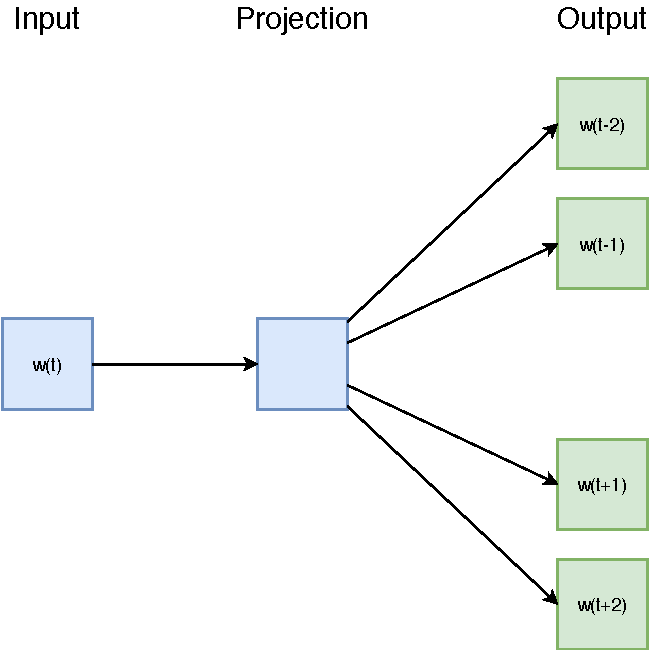
\includegraphics[scale=0.8]{skipgram}
\centering
\caption{Skip-gram model architecture.}
\label{fig:skipgram}
\end{figure}

It uses a skip-gram model (figure \ref{fig:skipgram}), proposed by Mikolov et al. in an earlier work \cite{mikolov2013a}, which is a prediction-based method.
The training objective of the skip-gram model is to find useful word representations for predicting the surrounding words in a sentence or a document.
It learns these representation by predicting the surrounding words for each word in a sentence within a defined max distance from the word.
Mikolov et al. show, that the produced representations exhibit linear structure that makes precise analogical reasoning possible \cite{mikolov2013}.

Given the computationally efficient model architecture of the skip-gram, the training times of Word2Vec are manageable even with huge amounts of data.

\subsubsection{GLoVe} \label{GLoVe}
Global Vectors for Word Representation (GLoVe) is a model to construct word representations.
It is a global log-bilinear regression model that combines the advantages from both Word2Vec-style local context window methods and global matrix factorization.
Training of GLoVe is done on aggregated global word-word co-occurrence statistics \cite{pennington2014}.

Given the same corpus and equal compute, Pennington et al. show that it outperforms Word2Vec and achieves better results faster \cite{pennington2014}, although Levy et al. \cite{levy2015} came to the opposite conclusion after careful testing.

\subsubsection{fastText} \label{fastText}
fastText is an open-source library for learning word embeddings and text classification.
It builds on the work of Word2Vec and improves on the skip-gram model by incorporating character n-grams in it.
Words are now represented as a sum of n-gram vectors instead of a single vector.
This is especially important for morphologically rich languages, such as Finnish, that contain many word forms that occur rarely in the training corpus, which makes learning good word representations difficult \cite{bojanowski2017}.

Mikolov et al. show that fastText significantly outperforms GLoVe on a number of tasks \cite{mikolov2017}.


\section{Training} \label{Training}
The goal of a neural network is to return a function $f()$ that accurately maps input examples to their labels.
To make it more precise, a \textit{loss function} is introduced to quantify the loss suffered when predicting examples in the training set.
A loss function assigns a numerical score to predicted outputs given the expected, true outputs.
The function is bounded from below such that the minimum value is only attainable in cases where the prediction is correct.
The goal of the training algorithm is then to minimize the average loss over all training examples \cite{goldberg2017}.

Attempting to minimize the loss at all costs may result in \textit{overfitting} the training data, thus a soft restriction on the loss function is applied in the form of a \textit{regularization term}, which tracks the ``complexity'' of parameters.
Thus the objective of the optimization problem becomes keeping a balance between low loss and low complexity \cite{goldberg2017}.

\subsection{Loss functions}\label{Loss functions}
\subsubsection{Binary cross entropy loss}\label{Binary cross entropy loss}
Binary cross entropy loss, also referred to as \textit{logistic loss} is a loss function used in binary classification with conditional probability outputs.
A set of two target classes labeled 0 and 1 is assumed, with a correct label $y\in{}\{0,1\}$.
The output of the classifier, $\tilde{y}$, is transformed to the range $[0, 1]$ using the sigmoid function $\sigma{}(x)=1/(1+e^{-x})$, and is interpreted as the conditional probability $\hat{y}=\sigma{}(\tilde{y}) = P(y=1|x)$.
The rule for prediction is:
\begin{equation}
prediction =
\begin{cases}
  \  0,\ \ \hat{y}\ <\ 0.5\\
  \ 1,\ \ \hat{y}\ \geq \ 0.5\\
\end{cases}
\end{equation}

The network maximizes the log conditional probability $\log\ P(y = 1|x)$ for each training example $(x,y)$.
Logistic loss is defined as:
\begin{equation}
  L_{logistic}\ (\hat{y},y)=-y\log\ \hat{y}-(1-y)\log\ (1-\hat{y}).
\end{equation}

The logistic loss is useful when we want the network to produce class conditional probability for a binary classification problem.
It is assumed that the output layer is transformed using the sigmoid function when using the logistic loss \cite{goldberg2017}.

\subsubsection{Categorical cross-entropy loss}\label{Categorical cross-entropy loss}
The categorical cross-entropy loss is a loss function that is used when a probabilistic interpretation of the scores is desired.
Let $y=y_{[1]},\ldots{},y_{[n]}$ be a vector representing the true multinomial distribution over the labels $1,\ldots{},n$, and let  $\hat{y}=\hat{y}_{[1]},\ldots{},\hat{y}_{[n]}$ be the linear classifier’s output transformed by the \textit{softmax} function, and represent the class membership conditional distribution $\hat{y}_{[i]} = P(y=i|x)$.
The softmax function forces the values of the output to be positive and sum to 1, thus making the output interpretable as a probability distribution.

The categorical cross entropy loss measures the dissimilarity between the true label distribution $y$ and the predicted label distribution $\hat{y}$, and is defined as cross entropy:
\begin{equation}
  L_{cross-entropy}\ (\hat{y},y)=-\sum_{i}y_{[i]}\log (\hat{y}_{[i]}).
\end{equation}

The case when each training example has only a single correct class assignment is called hard classification.
In such cases y is a one-hot vector representing the true class, and the cross entropy can be simplified to:
\begin{equation}
  L_{cross-entropy(hard classification)}\ (\hat{y},y)=-\log(\hat{y}_{[t]}),
\end{equation}
where $t$ is the correct class assignment.
This equation attempts to set the probability mass assigned to the correct class $t$ to 1.
Increasing the mass assigned to the correct class means decreasing the mass assigned to all the other classes given that the scores $\hat{y}$ have been transformed using the softmax function to be non-negative and sum to one.

The cross-entropy loss is widely used in log-linear models and neural networks.
It produces a multi-class classifier which predicts a distribution over all possible labels in addition to predicting the best class label.
When using the cross-entropy loss, it is assumed that the classifier’s output is transformed using the softmax function \cite{goldberg2017}.



\subsubsection{Ranking losses}\label{Ranking losses}
Margin-based ranking loss can be used in cases where supervision is not given as labels but as pairs of correct and incorrect samples $x$ and $x'$, and where the goal is to give a higher score to correct items.
Such a situations may occur when the training set consists of only positive examples and the generation of negative examples is done by corrupting positive ones.
Margin-based ranking loss is defined as follows for a pair of correct and incorrect samples:
\begin{equation}
  L_{ranking(margin)}(x,x')=\max(0, 1 - (f(x) - f(x'))),
\end{equation}
where $f(x)$ is the score assigned by the classifier for input vector $x$.
The objective of the function is to rank correct inputs above incorrect ones with a margin of at least 1.

Ranking loss is used in language tasks such as deriving pre-trained word embeddings (section \ref{Embeddings}) given a correct and corrupted word sequence, and the goal being to rank the correct sentence over the corrupt one \cite{goldberg2017}.


\subsection{Stochastic Gradient Descent}

Stochastic gradient descent (SGD) is a general optimization algorithm which powers nearly everything in deep learning.
The goal of the algorithm is to minimize the total loss over the training set by repeatedly sampling a training example and computing the gradient of the error on the example \cite{goldberg2017}.

Sampling each individual example and calculating a gradient for them quickly becomes infeasible when training set sizes are large, thus SGD uses \textbf{minibatching} to draw a uniform set of examples at a time from the training set to compute a gradient for.
The gradient is then propagated though the network and a new gradient is calculated from the next minibatch \cite{goodfellow2016}.

\textit{Learning rate} is a parameter that defines the amount that the weights of the network are updated with each gradient.
It is a small positive value, usually in the range $[0, 1]$.

Gradient descent has been regarded as slow or unreliable in the past.
Nowadays we know that it works great with neural networks even though it is not guaranteed that the algorithm will arrive even at a local minimum in a reasonable amount of time.
It however finds a very low value for the cost function quickly enough \cite{goodfellow2016}.

In addition to SGD, there exists other optimization algorithms which are used nowadays such as Adam \cite{kingma2017}, which is designed to define the learning rate on a minibatch basis.
Algorithms such as SGD+momentum \cite{polyak1964} are variants of SGD where the accumulated previous gradients affect the current update.

\section{Architectures} \label{Architectures}
\subsection{Recurrent Neural Network} \label{Recurrent Neural Network}

\begin{figure}[t]
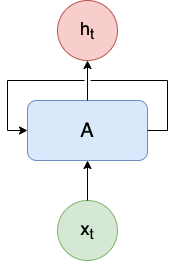
\includegraphics[scale=1]{rnnloop}
\centering
\caption{An RNN-module which illustrates the recurrent nature of the model}
\label{fig:rnnloop}
\end{figure}

Recurrent Neural Networks (RNN) are networks that process an input sequence one token at a time and maintain a state in its hidden units that contains information about the past elements in the sequence.
This approach has been proven to work well with tasks that contain sequential input such as speech, language and music \cite{lecun2015}.
Figure \ref{fig:rnnloop} shows the basic methodology behind an RNN: a chunk of neural network, A, looks at the input $x_t$ and outputs a value $h_t$. The output value is looped back as a second input value which allows for information to be passed from one step to the other.

\begin{figure}[t]
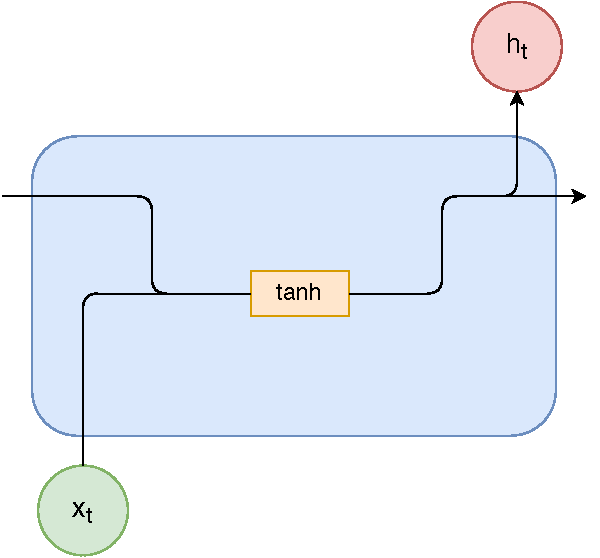
\includegraphics[scale=0.9]{rnn}
\centering
\caption{The insides of an RNN}
\label{fig:rnn}
\end{figure}

Figure \ref{fig:rnn} shows a visualization of the insides of an RNN module which is quite simple in practice. $x_t$ represents an input at timestep $t$, $tanh$ is a function that returns the hyperbolic tangent of the input and $h_t$ is the hidden state of the network at timestep $t$.
First the hidden state from the previous timestep and the current input value are added to each other after which the sum is fed into the $tanh$ function.
$tanh$ essentially squishes the input value between -1 and 1 to keep the values from exploding due to repeated multiplication.
The output of tanh is the new hidden state, the memory of the network, which is then fed to the next timestep.


The training of an RNN happens by using a variant of backpropagation called \textit{backpropagation through time} (bptt) which is a generalization of backpropagation for networks which store the activations of units while going forward in time \cite{rumelhart1985}.
The backward gradient update pass is thus also backward in time and recursively computes the required gradients with the saved activations.
It is easy to see how this works when the different timesteps of an RNN are unrolled and displayed as if they combine to make a single neural network with multiple layers (fig \ref{fig:rnn}).


RNNs have difficulties maintaining long-term dependencies when processing lengthy input sequences that originates from the \textit{vanishing gradients} problem \cite{bengio1994}:
During backpropagation gradients, with which the weights of the network are updated, change as they are applied backwards through time.
A small change to a layer before means an even smaller change in the current layer.
On the contrary, gradients with big changes tend to ``blow up''.
This means that the earlier layers in the network either stop learning since they only receive small gradient updates or their weights oscillate due to big changes \cite{hochreiter1997}.
In an RNN this problem is magnified due to backpropagation being applied to each time step.

\subsection{LSTM} \label{LSTM}
Long short-term memory (LSTM) is a recurrent network architecture proposed by Hochreiter and Schmidhuber in 1997 \cite{hochreiter1997}.
LSTM was designed to combat the vanishing gradients problem that is especially prevalent in RNNs.
LSTMs work exceptionally well on a large variety of problems and are widely used nowadays.

\begin{figure}[t]
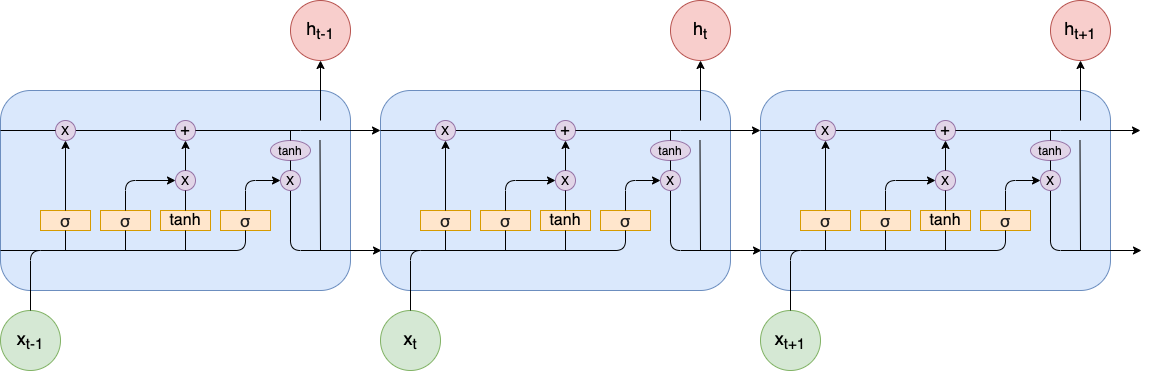
\includegraphics[scale=0.9]{lstm}
\centering
\caption{Long short-term memory network}
\label{fig:lstm}
\end{figure}

Figure \ref{fig:lstm} illustrates an lstm module. Each line carries a vector, merging lines denote concatenation, forking lines denote copying of the vector and each copy going to different directions, orange boxes are learned neural network layers and purple circles represent pointwise operations such as multiplication, addition and hyperbolic tangent.
In addition to keeping track of the hidden state of the network, LSTM adds another state called cell state that is denoted by the horizontal line running through the top of the figure.
Information is added and removed to the cell state by gates that are made up of sigmoid ($\sigma$) neural net layers and pointwise multiplication operations.
A sigmoid neural net layer takes as input the concatenation of the previous hidden state $h_{t-1}$ and the current input $x_t$ and output a vector of values between 0 and 1 to describe how much of each value is to be let through.
A value of 1 lets everything through while a 0 lets nothing through.
An LSTM has three of these gates.
From left to right, the first gate forms the forget gate layer which decides what data to keep and what to discard from the previous cell state.
Next, the data to add to the cell state is decided with a combination of a $sigmoid$ layer and a $tanh$ layer. The $tanh$ layer outputs new candidate values and the $sigmoid$ layer decides which of them to add to the cell state.
Finally, the last layer determines the output (hidden state) of the cell by taking the current cell state's values and applying a $tanh$ function to push the values between -1 and 1 and multiplying them with the output of the $sigmoid$ gate.
The new cell state and hidden state are then passed on to the next time step.

The LSTM architecture described above is considered a standard version of LSTM, but other variants exist too.
One popular variant of LSTM introduced by Gers \& Schmidhuber \cite{gers2000a} adds peephole-connections that allow the gate layers to look at the cell state.
Another variant called the \textbf{Gated Recurrent Unit} (GRU, figure \ref{fig:gru}), introduced by Cho, et al. \cite{cho2014}, simplifies the model by combining the forget and input gates into a single update gate.

\begin{figure}[t]
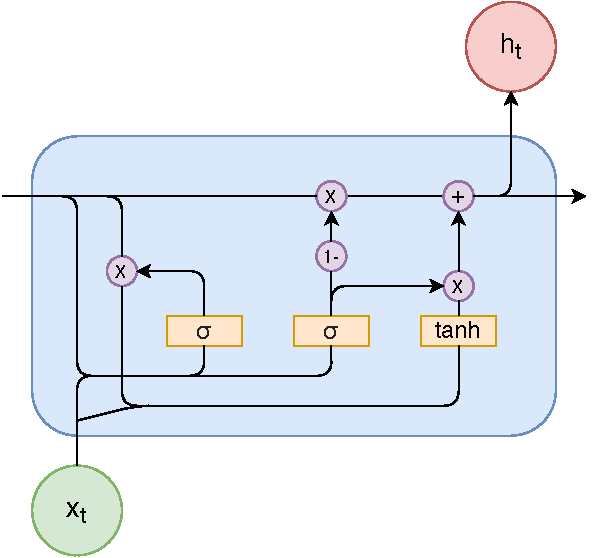
\includegraphics[scale=0.9]{gru}
\centering
\caption{Gated Recurrent Unit}
\label{fig:gru}
\end{figure}

\subsection{Transformer} \label{Transformer}
RNNs, as presented before, are inherently sequential in nature.
They take an input at timestep $t$ and compute a hidden state $h_t$ with knowledge from the previous hidden state $h_{t-1}$.
This sequentiality prohibits efficient parallelization within training examples since one has to come before the other in training.
Parallelization across examples is also critically constrained by memory at longer sequence lengths.
In addition to this, RNNs suffer from the so-called \textit{vanishing gradient problem} which is exacerbated at longer sequence lengths \cite{vaswani2017}.

Attention is a mechanism that allows the modeling of dependencies without regard for distance in input or output sequences.
It has been used in conjunction with recurrent neural networks to achieve good results, but using it with RNNs somewhat limits the power of attention since the model is still constrained by the aforementioned problems of RNNs.
Thus Vaswani et al. proposed a novel architecture in 2017, the Transformer, to combat these limitations.
The Transformer has been the foundation of neural networks that have achieved state-of-the-art results in various language-related tasks in the last couple of years \cite{vaswani2017}.

The Transformer consists of an encoder, which maps an input sequence of tokens to a sequence of continuous representations, and a decoder, which takes a continuous representation and generates an output sequence.
The output sequence is generated one token at a time while taking the previous generated tokens as additional input.

\begin{figure}[t]
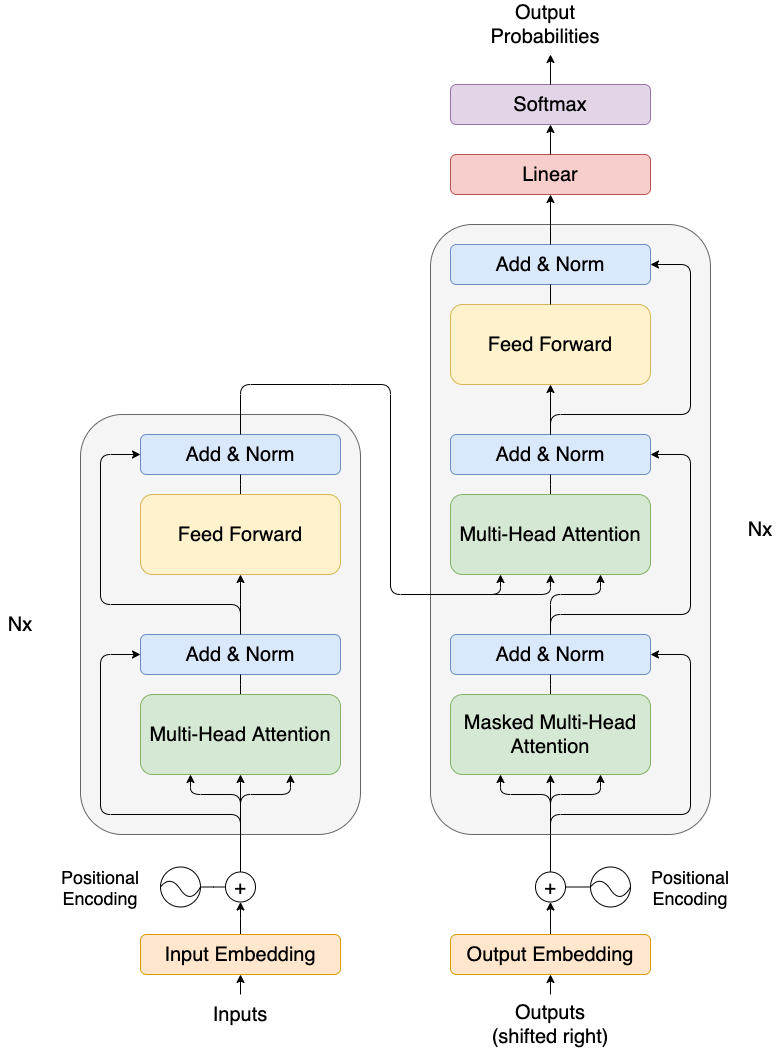
\includegraphics[scale=0.5]{transformer}
\centering
\caption{The Transformer, from Vaswani et al. 2017 \cite{vaswani2017}}
\label{fig:transformer}
\end{figure}

The overall architecture of the Transformer is shown in Figure \ref{fig:transformer}, with the left side of the figure representing the encoder and the right side the decoder.
The encoder is composed of six identical layers stacked on top of each other.
Each layer consists of two sub-layers; a multi-head self-attention mechanism and a fully connected feed-forward network.
Residual connections \cite{he2016} are used around each sub-layer to shortcut the sub-layers while training.
This leads to faster training times and a more robust model as the connections are gradually restored during training.
Finally, layer normalization is applied to the output of the sub-layer as $LayerNorm(x+Sublayer(x))$, where $Sublayer(x)$ refers to the function implemented by the sub-layer.
Due to the residual connections, all sub-layers and embedding layers have to produce outputs of the same dimensionality.
Thus in the Transformer the dimensionality is defined as $d_{model}=512$.

The decoder is also composed of six identical layers but additionally includes a third sub-layer, which applies multi-head attention over the output of the encoder stack.
The self-attention sub-layer in the decoder stack is also modified to prevent positions from attending to subsequent positions.
Thus predictions for position $i$ can only depend on the outputs before $i$.

Attention can be described as a function of mapping a query and a set of key-value pairs to an output.
The query, keys, values and output are all vectors.
The output is a weighted sum of the values, where the weight of each value is defined by a compatibility function of the query with the corresponding key.
The particular version of attention in the Transformer is called \textit{Scaled Dot-Product Attention} in which the input consists of queries and keys of dimension $d_k$ and values of dimension $d_v$.
The dot products of queries with all keys are computed first, denoted by $QK^T$ in equation \ref{eq:attention}.
The results are divided by $\sqrt{d_k}$ and then a softmax function is applied to obtain the weights on the values \cite{vaswani2017}.


\begin{equation}
  Attention(Q,K,V)=softmax(\dfrac{{QK^T}}{{\sqrt{d_k}}})V\label{eq:attention}
\end{equation}

Instead of using a single attention function over all the keys, values and queries with dimension $d_{model}$, the Transformer uses so-called \textit{Multi-Head Attention} to linearly project the keys, values and queries $h$ times to $d_k$, $d_k$ and $d_v$ dimensions.
The attention function is then applied in parallel to all these projected versions, yielding $d_v$-dimensional outputs.
These outputs are then concatenated and projected to achieve the final result.
This allows the model to jointly attend to information from different representation subspaces at different positions.
In the Transformer, 8 parallel attention heads are used \cite{vaswani2017}.

Attention is used in three different ways in the Transformer.
In encoder-decoder attention, where the output of the encoder is used in the decoder, the queries come from the previous decoder layer and the keys and values come from the output of the encoder, and in encoder and decoder self-attention.
In encoder self-attention all the queries, keys and values come from the output of the previous encoder layer, thus each position in the encoder can attend to all positions in the previous encoder layer.
Decoder self-attention similarly receives its input from the previous decoder layer's output, but doesn't allow attention over all the positions but only up to and including the current position.
This is achieved by masking out all the input values of the softmax corresponding to illegal connections.

The decision to use self-attention was made based on three requirements: to minimize the total computational complexity of each layer, to maximize the amount of parallelizable computation and to minimize the path length between long-range dependencies.
A side benefit of self-attention is more interpretable models as attention distributions can be inspected and tested with different examples to gain insight into the behaviour of individual attention heads \cite{vaswani2017}.

\subsection{Other architectures} \label{Other architectures}
\subsubsection{Autoencoder}\label{Autoencoder}
Autoencoders are neural networks that are trained to attempt to copy its input to its output.
They compress the input into a lower-dimensional representation after which they attempt to reconstruct the original input from this representation.
An autoencoder that succeeds at a perfect copy is not very useful, thus they are designed to be unable to learn to copy perfectly.
Because the model has to prioritize which aspects of the input should be copied, it often learns useful properties of the data \cite{goodfellow2016}.


\begin{figure}[t]
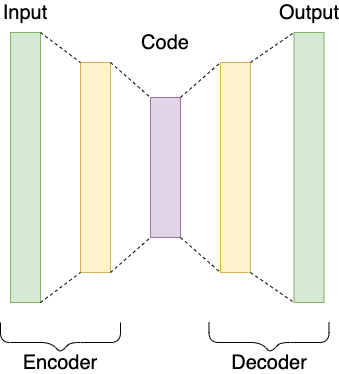
\includegraphics[scale=1]{autoencoder}
\centering
\caption{The autoencoder}
\label{fig:autoencoder}
\end{figure}

An autoencoder consists of three components: an encoder, code and a decoder.
The encoder compresses the input and produces the code, the decoder reconstructs the input from the code.
Figure \ref{fig:autoencoder} illustrates the simple architecture of the autoencoder.
Both the encoder and the decoder are fully connected feedforward networks and are essentially mirror images of each other.
The only requirement of the autoencoder is that the input and output dimensions are the same.

Autoencoders have traditionally been used for dimensionality reduction or feature learning \cite{goodfellow2016}.
For natural language processing, Variational Autoencoders \cite{kingma2014} have been used for generative document modelling and supervised question answering \cite{miao2016}.



\subsubsection{Convolutional Neural Network}\label{CNN}
\begin{figure}[t]
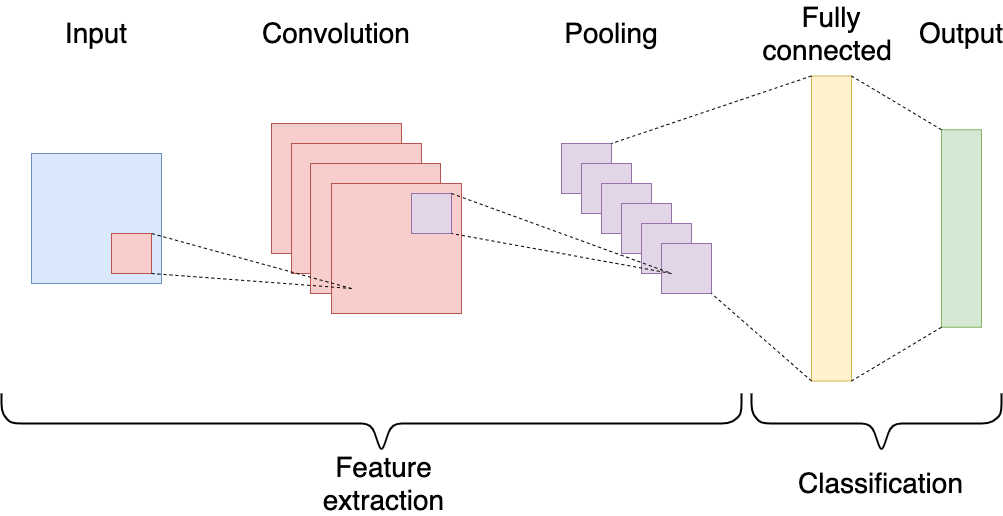
\includegraphics[scale=0.55]{cnn}
\centering
\caption{A convolutional neural network for classification}
\label{fig:cnn}
\end{figure}
Convolutional Neural Networks (CNN) are networks that incorporate convolutional and pooling layers into a neural network.
CNN's have four key ideas that take advantage of the properties of signals: shared weights, pooling, local connections and the use of many layers.
A typical CNN (Figure \ref{fig:cnn}) is structured as a series of stages.
The first stages are composed of convolutional layers and pooling layers.
Convolutional layers try to detect local conjunctions of features from the previous layer.
A convolutional layer's units are organized in feature maps, within which each unit is connected to local patches in feature maps of the previous layer.
These connections are weighted and the weights are contained in a filter bank, that is shared within all the units of a feature map.
Every feature map thus has it's own filter bank.
The role of the pooling layers is to merge semantically similar features into one.
They reduce the dimension of the representation in an effort to make the network more robust against small shifts and distortions in the data.
Stacks of convolutions and pooling are finally followed by fully-connected layers that are trained to output the result \cite{lecun2015}.


Convolutional neural networks have been used for a multitude of tasks in natural language processing in the past such as sentiment classification and sentence modeling \cite{kalchbrenner2014}.


\section{Modern models} \label{Modern models}

\subsection{ULMFiT} \label{ULMFiT}
Universal Language Model fine-tuning (ULMFiT) is a transfer learning based methodology for text classification which posted state-of-the-art results when it was published in 2018.
It consists of firstly pre-training a language model on a general-domain corpus and then fine-tuning it on a classification task.
This idea of first pre-training on a large general corpus and then fine-tuning it has been tried before, but has proven to be a challenging task due to it requiring millions of in-domain documents to achieve good performance \cite{dai2015}.
With ULMFiT Howard et al. proposed novel training techniques to make the training feasible even with a small corpus \cite{howard2018}.

ULMFiT is a \textit{universal} method in that it uses a single architecture and training process, requires no custom feature engineering, works across tasks with variable document sizes and label types, and doesn't require additional in-domain documents or labels \cite{howard2018}.

ULMFiT uses a 3-layer weight-dropped long shot-term memory (AWD-LSTM) network, proposed by Merity et al. \cite{merity2017}, which is a recurrent neural network (RNN).
AWD-LSTM is a vanilla LSTM with various regularization and optimization strategies such as DropConnect \cite{wan}, which prevents over-fitting by randomly dropping connections between the recurrent hidden to hidden weight matrices, and averaged gradient descent as its optimization algorithm.

The training begins with pre-training a general-domain language model with unlabeled text data to capture the general properties of language.
This initial training step is the most expensive in the whole method but only needs to be done once.

After the general language model is trained, it is fine-tuned with the target task data.
This fine-tuning converges faster than the initial pre-training since the model needs to only adapt to the idiosyncrasies of the fine-tuning data.
This allows the training of robust language models even with small datasets.
ULMFiT uses \textit{discriminative fine-tuning} and \textit{slanted triangular learning rates} for the fine-tuning step of the language model.
With discriminative fine-tuning, instead of using a single learning rate for all the layers in the model, each layer is fine-tuned with a learning rate of its own.
The motivation for this comes from the fact that different layers capture different types of information, thus each layer should be fine-tuned for different amounts.
With slanted triangular learning rates, the learning rate is first linearly increased in order to get the model to quickly converge to a suitable region, and then linearly decreased to refine its parameters.

For the final step, two additional linear blocks are added to the end of the network, and the final classifier is fine-tuned with \textit{gradual unfreezing}.
Gradual unfreezing is used to prevent \textit{catastrophic forgetting} by unfreezing the layers of the model one by one, starting from the last.
Unfrozen layers are fine-tuned for one epoch after which the next layer is unfrozen until all the layers of the model have been unfrozen.
The whole model is then fine-tuned until convergence \cite{howard2018}.

Although outshined by BERT and other huge transformer-based models, ULMFiT is much fast to train and typically does not require a lot of data to get good results.



\subsection{BERT} \label{BERT}
Bidirectional Encoder Representations from Transformers (BERT) is a language representation model based on the Transformer \cite{vaswani2017} architecture (subsection \ref{Transformer}).
It uses a \textit{fine-tuning} based approach, in which all the pre-trained parameters are fine-tuned when applying pre-trained language representations to down-stream tasks, as opposed to a \textit{feature-based} approach, where the pre-trained representations are only used as additional features in a task-specific architecture.

Both the fine-tuning and feature-based approach share the same objective function during pre-training of learning general language representations by using unidirectional language models.
BERT uses a \textit{masked language model} (MLM) pre-training objective to achieve bi-directionality in context, thus allowing the model to see both left and right of the input token when training.
MLM randomly masks tokens in the input, and the objective is to predict the vocabulary id of the masked token based on its context.
BERT also uses a \textit{next sentence prediction} (NSP) task that jointly pre-trains text-pair representations \cite{devlin2019}.

As with ULMFiT, BERT also has a unified architecture across different tasks with a minimal difference between the pre-trained architecture and the final downstream one.
BERT's architecture is almost identical with the Transformer described in section \ref{Transformer}, the difference comes mainly in the number of layers (Transformer blocks), denoted as $L$, hidden size, denoted as $H$ and the number of attention heads, denoted as $A$.
Results for BERT performance was primarily reported for two sizes: $BERT_{BASE}$ (L=12, H=768, A=12, total parameters=110M) and $BERT_{LARGE}$ (L=24, H=1024, A=16, total parameters=340M).

BERT uses WordPiece embeddings \cite{wu2016}, essentially similar to SentencePiece embeddings (section \ref{SentencePiece}).
Pre-training happens by the two aforementioned unsupervised tasks: Masked language modeling and next sentence prediction.

In MLM, 15\% of all WordPiece tokens are randomly chosen and each chosen token has an 80\% chance to actually be masked, a 10\% chance to be replaced with a random token, and a 10\% chance to stay unchanged.
The reason for not always masking the chosen tokens is because the [MASK] token does not appear during fine-tuning, causing a mismatch between the two steps otherwise.

In NSP, training examples consist of two sentences $A$ and $B$.
50\% of the time $B$ is actually the next sentence that follows $A$ (label $IsNext$) and 50\% of the time it is a random sentence from the corpus (label $NotNext$).

With the use of the Transformer-architecture, WordPiece embeddings and two pre-training objectives that allow bidirectional context, BERT was able to exceed the state-of-the-art on multiple downstream tasks \cite{devlin2019}.

\subsection{ELECTRA} \label{ELECTRA}
Efficiently Learning an Encoder that Classifies Token Replacements Accurately (ELECTRA) is a further elaboration on the BERT model by Clark, et al. \cite{clark2020}
The primary motivation for ELECTRA is making pre-training more efficient given that training a full-sized BERT or any derivation of it (ALBERT, RoBERTa etc.) requires a considerable amount of compute and training data.
As described in the BERT chapter (chapter \ref{BERT}), BERT uses masked language modeling as a pre-training objective.
This MLM is inherently quite inefficient in its usage of the training data; only the masked tokens, approximately 15\% of the data, needs to be predicted.
As an alternative, ELECTRA proposes \textit{replaces token detection}, a pre-training task in which the model has to predict whether or not a token is the original token in the corpus or if it has been swapped for a token generated by a small masked language model.
This also solves the mismatch in BERT where the model sees [MASK] tokens during pre-training but not during fine-tuning.
ELECTRA trains the network as a discriminator rather than a generator, since it is predicting whether an input is corrupted or not.
This way ELECTRA learns from all the input tokens, rather than a small subset of them.

ELECTRA substantially outperforms MLM-based methods given the same amount of data and compute and works well even with relatively small amounts of compute \cite{clark2020}.
